\documentclass[25pt, a0paper, portrait, blockverticalspace=.5cm]{tikzposter}
\usepackage[utf8]{inputenc}
\usepackage{amssymb,amsfonts,amsmath,mathtext,mathtools}
\usepackage{xfrac}
\usepackage{enumitem}

\let\vec\oldvec
\newcommand{\vec}[1]{\boldsymbol{#1}}

\title{\parbox{\linewidth}
	{\centering
		ByPass optics design in NICA storage ring for experiment with polarized beams for EDM search\		
}}

\author{S. Kolokolchikov\textsuperscript{1}*, Y. Senichev\textsuperscript{2}, A. Aksentyev\textsuperscript{2}, \\A. Melnikov\textsuperscript{2}, 
		E. Syresin\textsuperscript{3}, V.Ladygin\textsuperscript{3}}
\institute{
	\textsuperscript{1} International Union of Pure and Applied Physics, Geneva, Switzerland\\
	\textsuperscript{2} Institute for Nuclear Research of the Russian Academy of Sciences, Moscow, Russia\\
	\textsuperscript{3} Joint Institute for Nuclear Researches, Dubna, Russia\\
	*sergey.bell13@gmail.com
}
\usetheme{Simple}
\usecolorstyle{Russia}
\colorlet{blocktitlefgcolor}{black}

\usepackage{caption}
\captionsetup{font=large}
\usepackage{multicol}
\setlength\columnsep{1.5cm}

\begin{document}

\maketitle


\begin{columns}
\column{.65}

\block{INTRODUCTION}{

\par NICA is mainly designed for experiments with heavy ions and polarized proton and deuteron beams at an
energy of the former about $13~$GeV. For these purposes, appropriate SPD and MPD detectors, as well as other
necessary implements, are installed in the straight sections. \textbf{Electric Dipole Moment} (EDM) experiment supposes to use deuterons at the energy of about $240~$MeV. 
To ensure the \textbf{"Quasi-Frozen Spin"} mode, E+B elements (namely, Wien Filters) are
required as well. Such elements can be placed in straight sections to compensate the arc spin rotation. 
\newline
\par For EDM measurement experiments, it is necessary to operate the NICA as a Storage Ring, and not in a collider
mode. To do this, it is proposed to install ByPass channels. Thus, it is possible to create a completely new
regular structure in a straight section. Creating ByPass channels will make it possible to engage NICA in various
experiments at once.
}
\block{EDM SEARCH}{

\section*{Frozen Spin}

\par To measure EDM, it is necessary to develop spin control methods. One of such methods is the concept of "Frozen Spin". And is a pure evident of T-BMT equations [1]. The magneto-optical structure of arcs implies the use of deflectors with both an electric and magnetic field. Thus, spin rotation in a magnetic field is compensated by an electric one (similarly for orbital motion). Thus, the spin retains its orientation during the entire time of rotation in the ring. However, the dipoles in the NICA arcs have only the magnetic field component. Thus, the implementation of the "Frozen Spin" concept is impossible in the NICA ring without appropriate modernisation and restructuring.

\section*{Quasi-Frozen Spin}

\par To carry out an experiment for EDM search, it becomes necessary to use an alternative spin control method, the concept of "Quasi-Frozen Spin" [2]. Unlike the "Frozen Spin" method, here the spin does not retain orientation throughout the entire period of circulation, but restores orientation on a straight section. This is possible by using elements with both E+B fields, which are called Wien Filters. The rotation of the spin in the arc by a certain angle is compensated by the corresponding rotation in the Wien Filter.  Also fields can be chosen to make zero-Lorentz force and do not disturb orbit and for this reason can be installed on straight sections. Thus, the polarimeters will detect the same orientation of the spin and for them it will be "frozen".

	}	

\block{BYPASS OPTICS DESIGN}{
	
		\begin{minipage}{0.51\linewidth}
			\begin{tikzpicture}
			\node (cone) at (0,0) {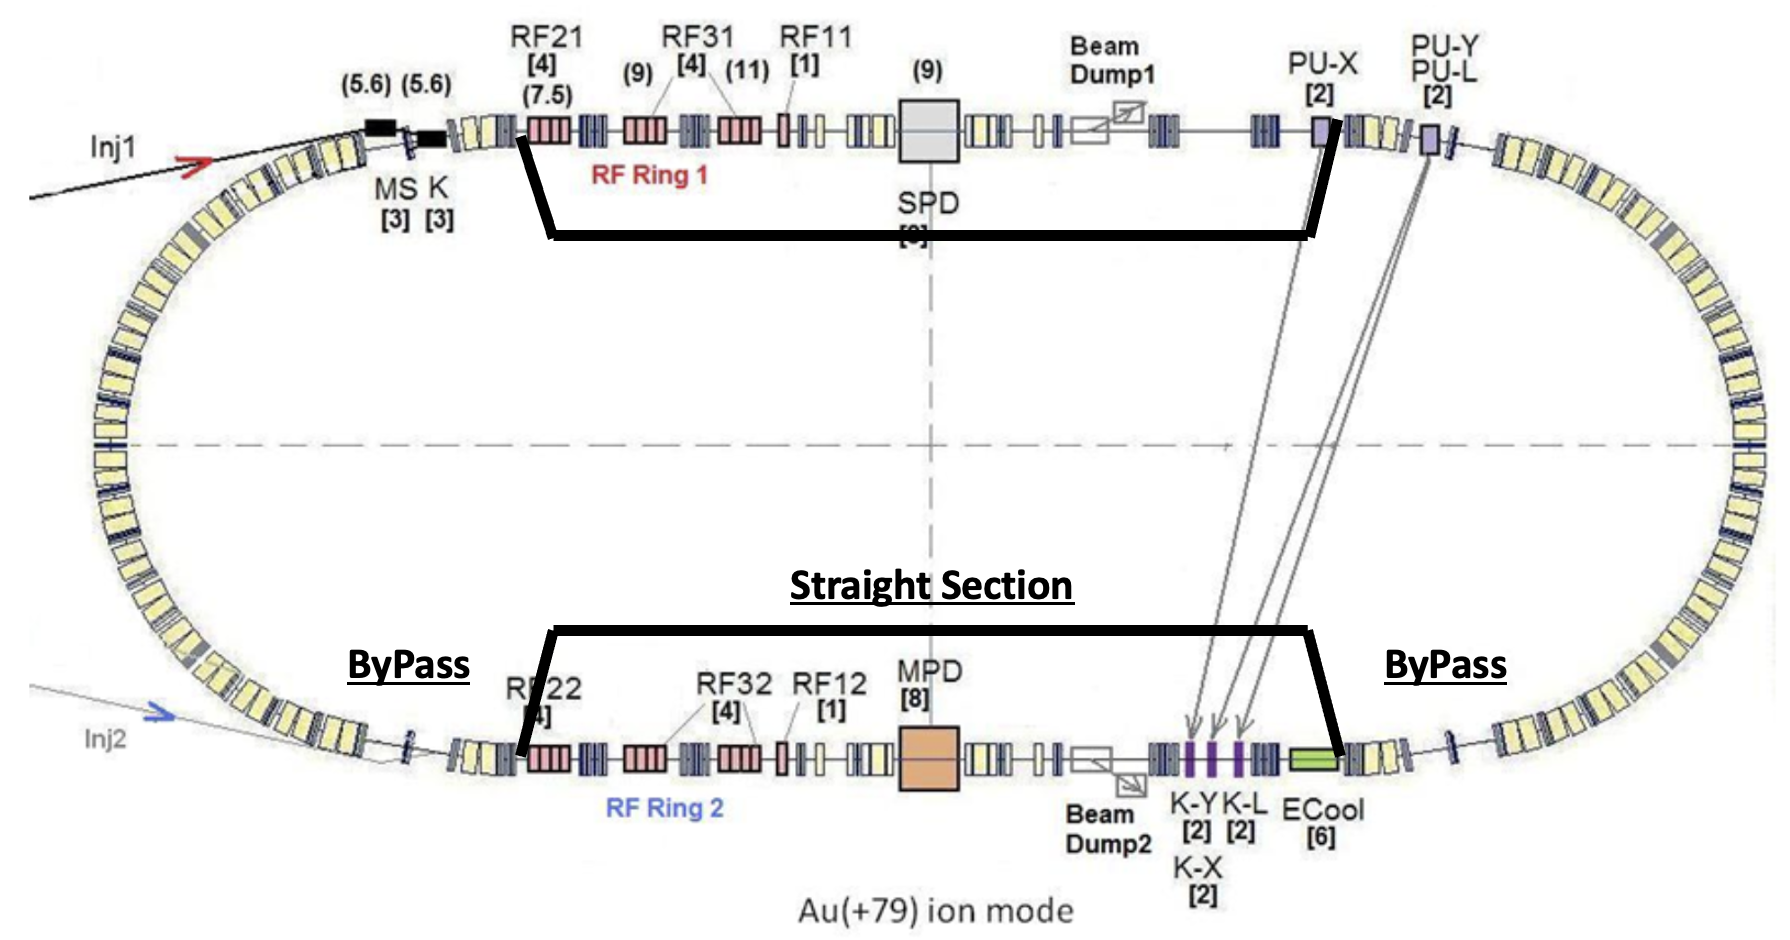
\includegraphics[width=\linewidth]{TEXPaper/img/MOPA072_f1-1.png}};
			\end{tikzpicture}
		\end{minipage}
		\begin{minipage}{0.49\linewidth}
			\par Designing the Storage Ring using ByPass based on NICA, 
we will take into account that the geometry of arcs is planned to remain unchanged. 
So that it is possible to use NICA for various experiments. 
In this case, an arc is a place with a non-zero dispersion, at the edges, 
both dispersion and its derivative take a zero value, thus the straight section has zero dispersion throughout. 
The total length of original NICA $L_{acc}~=~503.04~$m. One arc is $L_{arc}~=~142.15$~m. 
So, there is $(L_{acc}~-~2\cdot~L_{arc})/2~=~109.6$ m. available.
Only the gradients of the magnetic field in dipoles, quadrupoles and sextupoles will be changed for experiment purposes.
		\end{minipage}			
\newline
\newline
\newline
		\begin{minipage}{0.514\linewidth}
			\begin{tikzpicture}
			\node (cone) at (0,0) {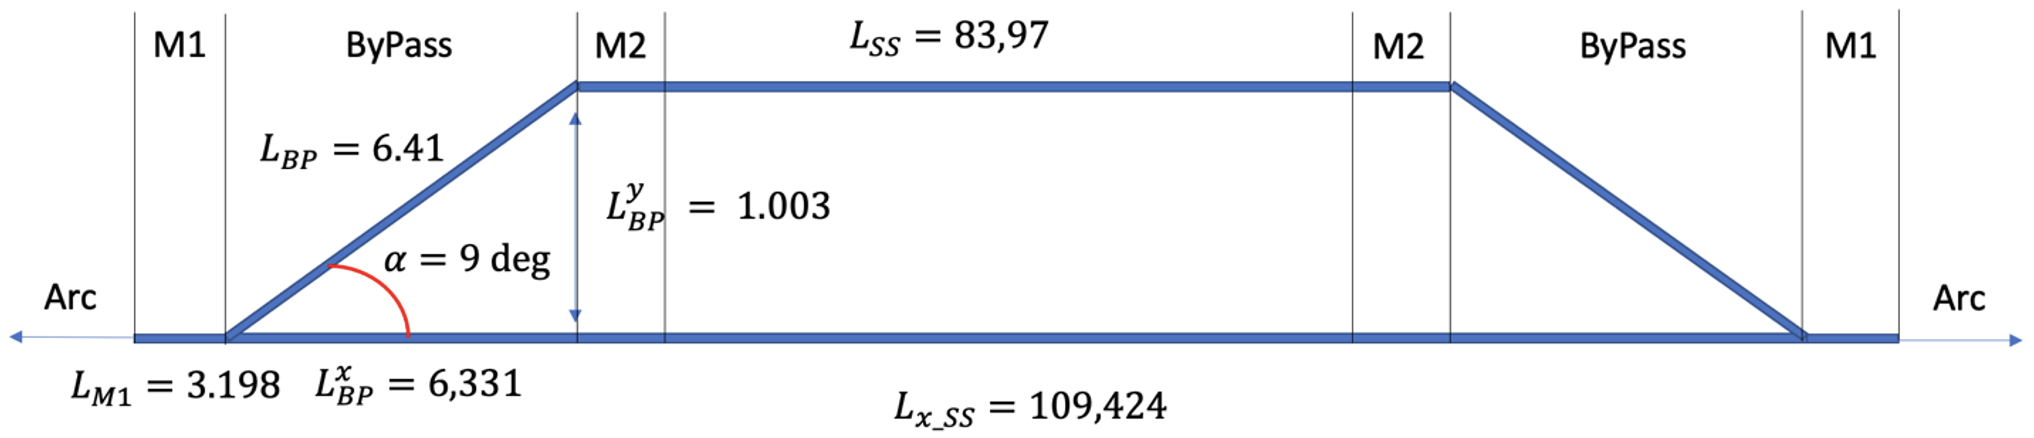
\includegraphics[width=\linewidth]{TEXPaper/img/MOPA072_f2-1.png}};
			\end{tikzpicture}
			\begin{tikzpicture}
			\node (cone) at (0,0) {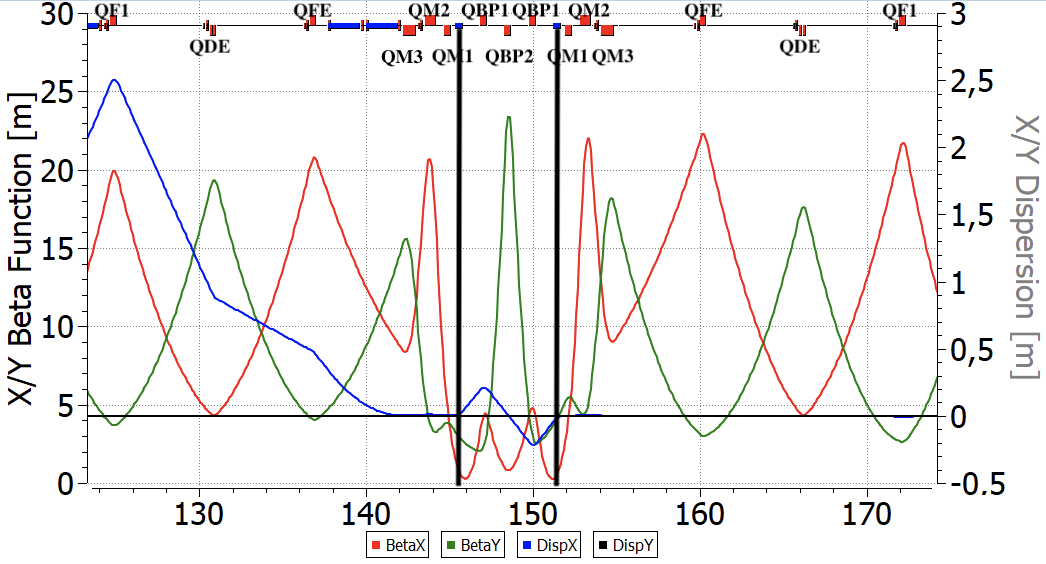
\includegraphics[width=\linewidth]{TEXPaper/img/MOPA072_f3-1.png}};
			\end{tikzpicture}
		\end{minipage}
		\begin{minipage}{0.486\linewidth}
			\begin{tikzpicture}
			\node (cone) at (0,0) {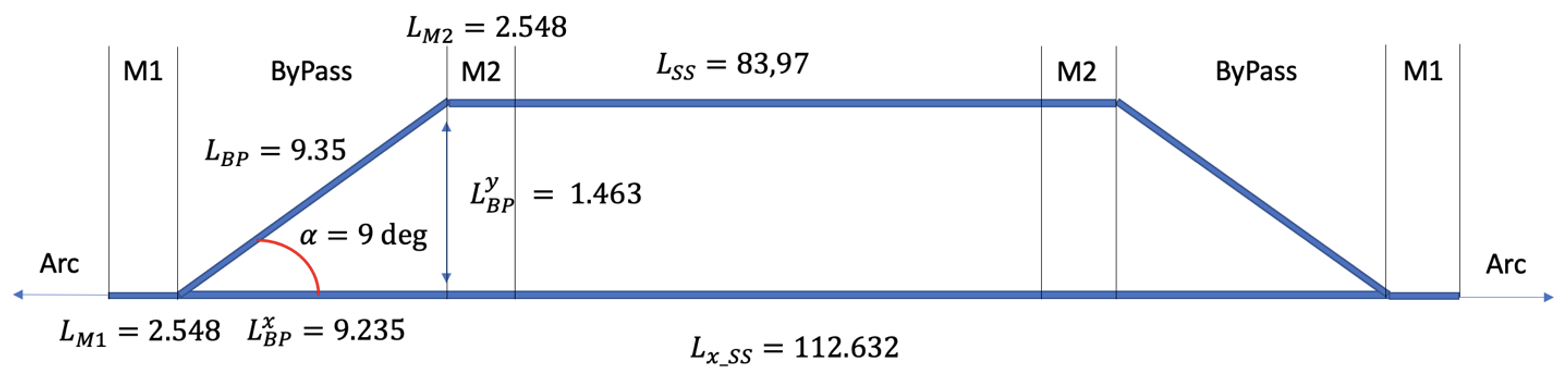
\includegraphics[width=\linewidth]{TEXPaper/img/MOPA072_f4-1.png}};
			\end{tikzpicture}
			\begin{tikzpicture}
			\node (cone) at (0,0) {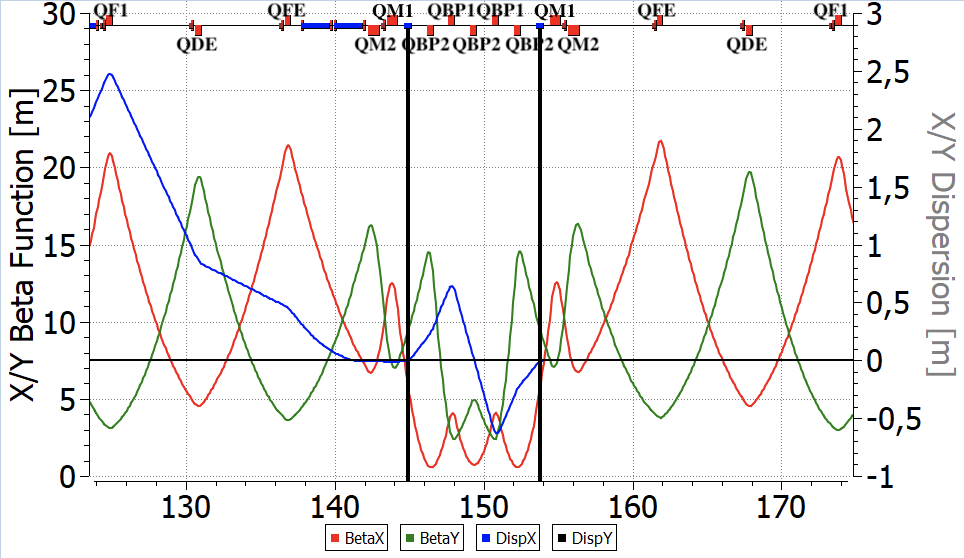
\includegraphics[width=\linewidth]{TEXPaper/img/MOPA072_f5-1.png}};
			\end{tikzpicture}
		\end{minipage}
\newline
\par For beam deflection into alternative straight section used dipole magnet and chosen to make a deviation by angle $\alpha~=~9^\circ$ and dipole strength at about $B_{BP}~=~1$~T with length $L^{BP}_{dip}~=~50$~m. If the alternative straight section is at a distance of 1 meter from the native ones, ByPass section length should be $L_{BP}~=~1~\text{m}/\sin{\alpha}\approx6.4~\text{m}$.}
	
\column{.35}
	\block{SPIN TRACKING}{
	
		\begin{minipage}{1.\linewidth}
			\begin{tikzpicture}
			\node (cone) at (0,0) {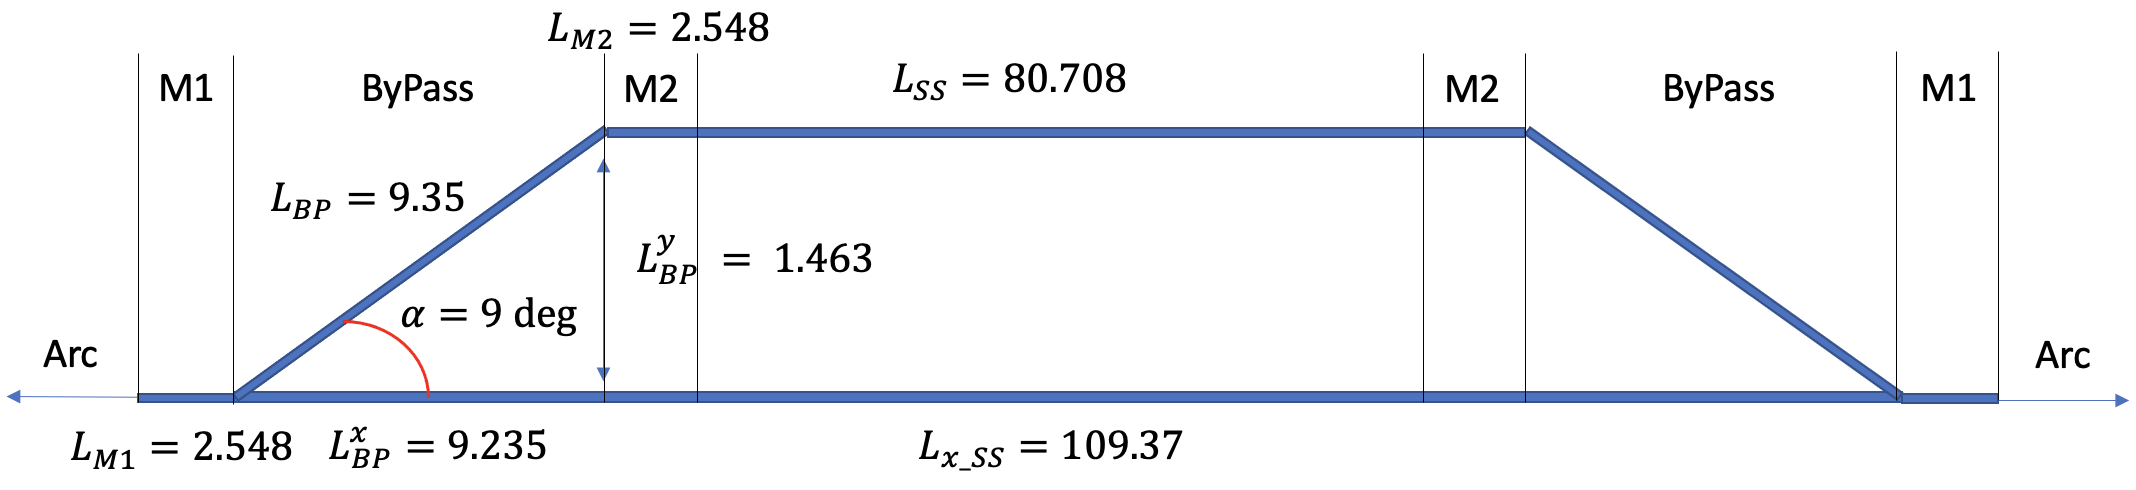
\includegraphics[width=\linewidth]{TEXPaper/img/MOPA072_f6-1.png}};
			\end{tikzpicture}
			\begin{tikzpicture}
			\node (cone) at (0,0) {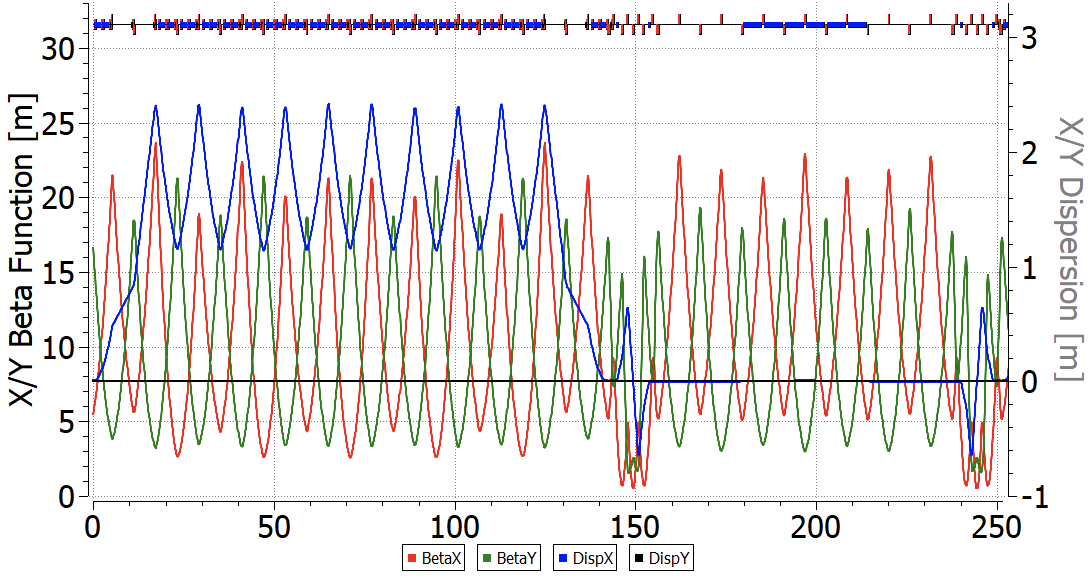
\includegraphics[width=\linewidth]{TEXPaper/img/MOPA072_f7-1.png}};
			\end{tikzpicture}
		\end{minipage}
		
 \par Based on the considered cases, we can get structure closely adopted to reality. Now, straight section is fully regular and shorter $L^{BP}_{SS}~=80.71$ m. ByPass consist from 5 quadrupoles and deflect beam by $1.46$~m. 

		\begin{minipage}{1.\linewidth}
			\begin{tikzpicture}
			\node (cone) at (0,0) {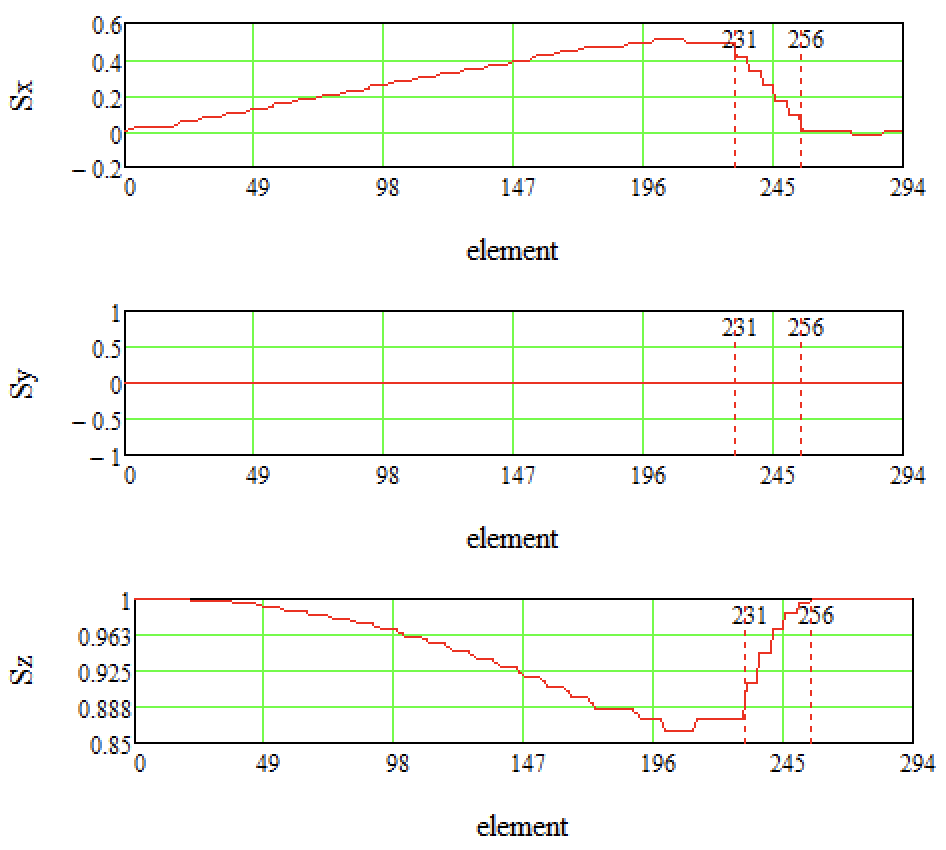
\includegraphics[width=\linewidth]{TEXPaper/img/MOPA072_f8-1.png}};
			\end{tikzpicture}
		\end{minipage}
\par All calculations and optimization of electric and magnetic fields in Wien Filters were made to get, first, zero Lorentz factor and, second, minimal spin-tune over the ring.}

	\block{CONCLUSION}{
\par For EDM experiments it is necessary to use NICA as a Storage Ring. 
For this reason modernization was considered by creation of an alternative straight sections parallel to the native ones by using ByPass channels.
Also straight sections have the ability to place special elements – Wien Filters to compensate spin rotation in the arcs.
As arcs remain unchanged, this allows to use NICA in various experiments.}

	\block{REFERENCES}{
	 
	\par [1] D. Anastassopoulos, V. Anastassopoulos, D. Babusci at al. AGS Proposal: Search for a permanent electric dipole moment of the deuteron nucleus at the $10^{-29}$ $e \cdot$cm level; BNL. — 2008.
	\par [2] Y. Senichev et al. Quasi-frozen spin concept of magneto-optical structure of NICA adapted to study the electric dipole moment of the deuteron and to search for the axion, Journal of Physics: Conference Series, 2420 (2023) 012052.\\ doi:10.1088/1742-6596/2420/1/012052
	\par [3] V. Lebedev, OptiM code, Private communication.\\ www.bdnew.fnal.gov/
	\par [4] 	COSY INFINITY. www.bmtdynamics.org/
	}
	
\end{columns}

\end{document}